% Seminar 1: Stochastic Processes and Stationarity
% Harvard-quality academic presentation
% Bachelor program, Bucharest University of Economic Studies

\documentclass[9pt, aspectratio=169, t]{beamer}

% Ensure content fits on slides
\setbeamersize{text margin left=8mm, text margin right=8mm}

%=============================================================================
% THEME AND STYLE CONFIGURATION
%=============================================================================
\usetheme{default}
% Using default theme for clean header/footer control

% Color Palette (matching Redispatch PDF)
\definecolor{MainBlue}{RGB}{26, 58, 110}
\definecolor{AccentBlue}{RGB}{26, 58, 110}
\definecolor{IDAred}{RGB}{205, 0, 0}
\definecolor{DarkGray}{RGB}{51, 51, 51}
\definecolor{MediumGray}{RGB}{128, 128, 128}
\definecolor{LightGray}{RGB}{248, 248, 248}
\definecolor{VeryLightGray}{RGB}{235, 235, 235}
\definecolor{KeynoteGray}{RGB}{218, 218, 218}
\definecolor{SectionGray}{RGB}{120, 120, 120}
\definecolor{FooterGray}{RGB}{100, 100, 100}
\definecolor{Crimson}{RGB}{220, 53, 69}
\definecolor{Forest}{RGB}{46, 125, 50}
\definecolor{Amber}{RGB}{181, 133, 63}
\definecolor{Orange}{RGB}{230, 126, 34}
\definecolor{Purple}{RGB}{142, 68, 173}

% Gradient background (exact Keynote 315° gradient: white to RGB 218,218,218)
\setbeamertemplate{background}{%
    \begin{tikzpicture}[remember picture, overlay]
        \shade[shading=axis, shading angle=315,
        top color=white, bottom color=KeynoteGray]
        (current page.south west) rectangle (current page.north east);
    \end{tikzpicture}%
}
% Fallback solid color for compatibility
\setbeamercolor{background canvas}{bg=}

\setbeamercolor{palette primary}{bg=MainBlue, fg=white}
\setbeamercolor{palette secondary}{bg=MainBlue!85, fg=white}
\setbeamercolor{palette tertiary}{bg=MainBlue!70, fg=white}
\setbeamercolor{structure}{fg=MainBlue}
\setbeamercolor{title}{fg=IDAred}
\setbeamercolor{frametitle}{fg=IDAred, bg=}
\setbeamercolor{block title}{bg=MainBlue, fg=white}
\setbeamercolor{block body}{bg=VeryLightGray, fg=DarkGray}
\setbeamercolor{block title alerted}{bg=Crimson, fg=white}
\setbeamercolor{block body alerted}{bg=Crimson!8, fg=DarkGray}
\setbeamercolor{block title example}{bg=Forest, fg=white}
\setbeamercolor{block body example}{bg=Forest!8, fg=DarkGray}
\setbeamercolor{item}{fg=MainBlue}

% Footer colors (override Madrid theme blue)
\setbeamercolor{author in head/foot}{fg=FooterGray, bg=}
\setbeamercolor{title in head/foot}{fg=FooterGray, bg=}
\setbeamercolor{date in head/foot}{fg=FooterGray, bg=}
\setbeamercolor{section in head/foot}{fg=FooterGray, bg=}
\setbeamercolor{subsection in head/foot}{fg=FooterGray, bg=}

% Bullet styles (apply everywhere including blocks)
\setbeamertemplate{itemize item}{\color{MainBlue}$\boxdot$}
\setbeamertemplate{itemize subitem}{\color{MainBlue}$\blacktriangleright$}
\setbeamertemplate{itemize subsubitem}{\color{MainBlue}\tiny$\bullet$}
\setbeamertemplate{itemize/enumerate body begin}{\normalsize}
\setbeamertemplate{itemize/enumerate subbody begin}{\normalsize}

% Item spacing - compact style
\setlength{\leftmargini}{10pt}       % Level 1: minimal indent
\setlength{\leftmarginii}{10pt}      % Level 2: minimal additional indent
% Compact list spacing (zero extra space before/after lists in blocks)
\makeatletter
\def\@listi{\leftmargin\leftmargini \topsep 0pt \parsep 0pt \itemsep 0pt}
\def\@listii{\leftmargin\leftmarginii \topsep 0pt \parsep 0pt \itemsep 0pt}
\makeatother

\setbeamertemplate{navigation symbols}{}

%=============================================================================
% CUSTOM HEADLINE
%=============================================================================
\setbeamertemplate{headline}{%
    \vskip10pt%
    \hbox to \paperwidth{%
        \hskip0.5cm%
        {\small\color{FooterGray}\renewcommand{\hyperlink}[2]{##2}\insertsectionhead}%
        \hfill%
        \textcolor{FooterGray}{\small\insertframenumber}%
        \hskip0.5cm%
    }%
    \vskip4pt%
    {\color{FooterGray}\hrule height 0.4pt}%
}

%=============================================================================
% CUSTOM FOOTER
%=============================================================================
\usepackage{fontawesome5}

\setbeamertemplate{footline}{%
    {\color{FooterGray}\hrule height 0.4pt}%
    \vskip4pt%
    \hbox to \paperwidth{%
        \hskip0.5cm%
        \textcolor{FooterGray}{\small Time Series Analysis and Forecasting}%
        \hfill%
        \raisebox{-0.1em}{%
            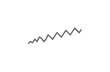
\begin{tikzpicture}[x=0.08em, y=0.08em, line width=0.4pt]
                \draw[FooterGray] (0,3) -- (1,4) -- (2,3.5) -- (3,5) -- (4,4) -- (5,6) -- (6,5.5) -- (7,4) -- (8,5) -- (9,7) -- (10,6) -- (11,5) -- (12,6.5) -- (13,8) -- (14,7) -- (15,6) -- (16,7.5) -- (17,9) -- (18,8) -- (19,7) -- (20,8.5) -- (21,10) -- (22,9) -- (23,8) -- (24,9.5);
            \end{tikzpicture}%
        }%
        \hskip0.5cm%
    }%
    \vskip6pt%
}

%=============================================================================
% PACKAGES
%=============================================================================
\usepackage[utf8]{inputenc}
\usepackage[T1]{fontenc}
\usepackage[english]{babel}
\usepackage{amsmath, amssymb, amsthm}
\usepackage{mathtools}
\usepackage{bm}
\usepackage{tikz}
\usetikzlibrary{arrows.meta, positioning, shapes, calc, decorations.pathreplacing, shadings}
\usepackage{booktabs}
\usepackage{multirow}
\usepackage{array}
\usepackage{graphicx}
\usepackage{hyperref}
\usepackage{colortbl}
\hypersetup{colorlinks=true, linkcolor=MainBlue, urlcolor=MainBlue}
\graphicspath{{../../logos/}{../../charts/}}
\hfuzz=2pt  % Suppress tiny overfull warnings (<2pt)
\vfuzz=2pt  % Suppress tiny vertical overfull warnings (<2pt)

%=============================================================================
% QUANTLET COMMAND
%=============================================================================
\newcommand{\quantlet}[2]{%
    \hfill\href{#2}{%
        \raisebox{-0.15em}{\includegraphics[height=0.7em]{ql_logo.png}}%
        \textcolor{MainBlue}{\tiny\ #1}%
    }%
}

%=============================================================================
% CUSTOM COMMANDS
%=============================================================================
\newcommand{\E}{\mathbb{E}}
\newcommand{\Var}{\text{Var}}
\newcommand{\Cov}{\text{Cov}}
\newcommand{\Corr}{\text{Corr}}
\newcommand{\R}{\mathbb{R}}
\newcommand{\RMSE}{\text{RMSE}}
\newcommand{\MAE}{\text{MAE}}
\newcommand{\MAPE}{\text{MAPE}}

\newcommand{\correct}{\textcolor{Forest}{\checkmark}}
\newcommand{\incorrect}{\textcolor{Crimson}{\texttimes}}

%=============================================================================
% CUSTOM TITLE PAGE
%=============================================================================
\defbeamertemplate*{title page}{hybrid}[1][]
{
    \vspace{0.2cm}
    % Logos row - top header (with clickable links)
    \begin{center}
        \href{https://www.ase.ro}{\includegraphics[height=1.0cm]{ase_logo.png}}\hspace{0.3cm}%
        \href{https://theida.net}{\includegraphics[height=1.0cm]{ida_logo.png}}\hspace{0.3cm}%
        \href{https://blockchain-research-center.com}{\includegraphics[height=1.0cm]{brc_logo.png}}\hspace{0.3cm}%
        \href{https://www.ai4efin.ase.ro}{\includegraphics[height=1.0cm]{ai4efin_logo.png}}\hspace{0.3cm}%
        \href{https://ipe.ro/new}{\includegraphics[height=1.0cm]{acad_logo.png}}\hspace{0.3cm}%
        \href{https://www.digital-finance-msca.com}{\includegraphics[height=1.0cm]{msca_logo.png}}%
    \end{center}

    \vspace{0.6cm}

    % Main title with Q logos on sides (with clickable links)
    \begin{center}
        \begin{minipage}{0.1\textwidth}
            \centering
            \href{https://quantlet.com}{\includegraphics[height=1.1cm]{ql_logo.png}}
        \end{minipage}%
        \begin{minipage}{0.78\textwidth}
            \centering
            {\LARGE\bfseries\usebeamercolor[fg]{title}\inserttitle}

            \vspace{0.3cm}

            {\usebeamerfont{subtitle}\usebeamercolor[fg]{title}\insertsubtitle}
        \end{minipage}%
        \begin{minipage}{0.1\textwidth}
            \centering
            \href{https://quantinar.com}{\includegraphics[height=1.1cm]{qr_logo.png}}
        \end{minipage}
    \end{center}

    \vspace{0.6cm}

    % Authors (left aligned)
    \hspace{0.5cm}{\usebeamerfont{author}\insertauthor}

    \vspace{0.3cm}

    % Institute/Affiliations (left aligned)
    \hspace{0.5cm}\begin{minipage}[t]{0.9\textwidth}
        \raggedright\small\insertinstitute
    \end{minipage}
}

%=============================================================================
% TITLE INFORMATION
%=============================================================================
\title[Time Series Analysis]{Time Series Analysis and Forecasting}
\subtitle{Seminar 1: Stochastic Processes and Stationarity}
\author[D.T. Pele]{Daniel Traian PELE}
\institute{Academia de Studii Economice din Bucure\c{s}ti\\
IDA Institute Digital Assets\\
Blockchain Research Center\\
AI4EFin Artificial Intelligence for Energy Finance\\
Academia Rom\^{a}n\u{a}, Institutul de Prognoz\u{a} Economic\u{a}\\
MSCA Digital Finance}
\date{}

\begin{document}

% Title page (no header/footer)
{
\setbeamertemplate{headline}{}
\setbeamertemplate{footline}{}
\begin{frame}
    \titlepage
\end{frame}
}

%=============================================================================
% SEMINAR OUTLINE
%=============================================================================
\begin{frame}{Seminar Outline}
    \textbf{\large Seminar structure:}

    \vspace{0.4cm}

    \begin{enumerate}
        \item[\textcolor{MainBlue}{\textbf{1.}}] \textbf{Quick Review} -- Key concepts summary
        \vspace{0.15cm}
        \item[\textcolor{MainBlue}{\textbf{2.}}] \textbf{Multiple Choice Quiz} -- Knowledge check
        \vspace{0.15cm}
        \item[\textcolor{MainBlue}{\textbf{3.}}] \textbf{True/False Questions} -- Conceptual checks
        \vspace{0.15cm}
        \item[\textcolor{MainBlue}{\textbf{4.}}] \textbf{Calculation Exercises} -- Applied practice
        \vspace{0.15cm}
        \item[\textcolor{MainBlue}{\textbf{5.}}] \textbf{Python Exercises} -- Coding practice
        \vspace{0.15cm}
        \item[\textcolor{MainBlue}{\textbf{6.}}] \textbf{Discussion Questions} -- Critical thinking
        \vspace{0.15cm}
        \item[\textcolor{MainBlue}{\textbf{7.}}] \textbf{AI-Assisted Exercises} -- Stationarity with AI
    \end{enumerate}
\end{frame}

%=============================================================================
% PART 1: QUICK REVIEW
%=============================================================================
\section{Quick Review}

\begin{frame}{Key Formulas}
    \begin{columns}[T]
        \begin{column}{0.48\textwidth}
            \textbf{Decomposition:}
            \begin{itemize}
                \item Additive: $X_t = T_t + S_t + \varepsilon_t$
                \item Multiplicative: $X_t = T_t \times S_t \times \varepsilon_t$
            \end{itemize}

            \vspace{0.3cm}

            \textbf{Exponential Smoothing:}
            \begin{itemize}
                \item SES: $\hat{X}_{t+1} = \alpha X_t + (1-\alpha)\hat{X}_t$
                \item Holt: adds trend $b_t$
                \item HW: adds seasonality $S_t$
            \end{itemize}
        \end{column}
        \begin{column}{0.48\textwidth}
            \textbf{Stationarity:}
            \begin{itemize}
                \item $\E[X_t] = \mu$ (constant)
                \item $\Var(X_t) = \sigma^2$ (constant)
                \item $\Cov(X_t, X_{t+h}) = \gamma(h)$
            \end{itemize}

            \vspace{0.3cm}

            \textbf{Random walk:}
            \begin{itemize}
                \item $X_t = X_{t-1} + \varepsilon_t$
                \item $\Var(X_t) = t\sigma^2$ (grows with time)
            \end{itemize}
        \end{column}
    \end{columns}
\end{frame}

\begin{frame}{Summary: Concepts and Methods}
    \begin{center}
    \small
    \begin{tabular}{lll}
        \toprule
        \textbf{Concept} & \textbf{Key idea} & \textbf{When to use} \\
        \midrule
        Additive decomposition & Constant seasonal amplitude & Stable variance \\
        Multiplicative decomposition & Seasonality grows with level & Increasing variance \\
        SES & Level only ($\alpha$) & No trend, no seasonality \\
        Holt & Level + Trend ($\alpha, \beta$) & Trend, no seasonality \\
        Holt-Winters & Level + Trend + Seasonality & Trend and seasonality \\
        \midrule
        ADF Test & $H_0$: unit root & Test for non-stationarity \\
        KPSS Test & $H_0$: stationary & Confirm stationarity \\
        \midrule
        Differencing & Remove stochastic trend & Random walk, unit root \\
        Regression & Remove deterministic trend & Linear/polynomial trend \\
        \bottomrule
    \end{tabular}
    \end{center}
\end{frame}

%=============================================================================
% PART 2: MULTIPLE CHOICE QUIZZES
%=============================================================================
\section{Multiple Choice Quiz}

\begin{frame}{Quiz 1: Stationarity}
    \begin{alertblock}{Question}
        A random walk process $X_t = X_{t-1} + \varepsilon_t$ is:
    \end{alertblock}

    \vspace{0.4cm}

    \begin{enumerate}[A.]
        \item Strictly stationary
        \item Weakly stationary
        \item Non-stationary because variance grows with time
        \item Stationary after adding a constant
    \end{enumerate}

    \vspace{0.5cm}

    \begin{center}
        \textit{Answer on next slide...}
    \end{center}
\end{frame}

\begin{frame}{Quiz 1: Answer}
    \begin{exampleblock}{Answer: C -- Non-stationary because variance grows with time}
        For random walk: $X_t = \sum_{i=1}^{t} \varepsilon_i$
        \begin{itemize}
            \item $\E[X_t] = 0$ (constant mean -- OK)
            \item $\Var(X_t) = t\sigma^2$ (variance depends on $t$ -- NOT OK!)
            \item Variance is \textbf{not} constant $\Rightarrow$ violates the stationarity condition
                \begin{itemize}
                    \item \textbf{Solution}: differencing gives $\Delta X_t = \varepsilon_t$ --- stationary
                \end{itemize}
        \end{itemize}
    \end{exampleblock}
\end{frame}

\begin{frame}{Visual: Random Walk vs Stationary}
    \begin{center}
        \includegraphics[width=0.95\textwidth]{ch3_def_random_walk.pdf}
    \end{center}
    \vspace{-0.2cm}
    {\small
    \begin{itemize}\setlength{\itemsep}{0pt}
        \item Random walk trajectories wander unpredictably
        \item Variance grows linearly with time $\Rightarrow$ non-stationary
    \end{itemize}
    }
    \quantlet{TSA\_ch1\_random\_walk}{https://github.com/QuantLet/TSA/tree/main/TSA\_Ch1/TSA\_ch1\_random\_walk}
\end{frame}

\begin{frame}{Quiz 2: Unit Root Tests}
    \begin{alertblock}{Question}
        You run ADF and KPSS tests. ADF fails to reject $H_0$, and KPSS rejects $H_0$. What do you conclude?
    \end{alertblock}

    \vspace{0.4cm}

    \begin{enumerate}[A.]
        \item The series is stationary
        \item The series has a unit root (non-stationary)
        \item The results are inconclusive
        \item Additional tests are needed
    \end{enumerate}

    \vspace{0.5cm}

    \begin{center}
        \textit{Answer on next slide...}
    \end{center}
\end{frame}

\begin{frame}{Quiz 2: Answer}
    \begin{exampleblock}{Answer: B -- The series has a unit root (non-stationary)}
        \begin{itemize}
            \item ADF: $H_0$ = unit root. Fail to reject $\Rightarrow$ evidence FOR unit root
            \item KPSS: $H_0$ = stationary. Reject $\Rightarrow$ evidence AGAINST stationarity
            \item Both tests agree: the series is \textbf{non-stationary}
                \begin{itemize}
                    \item \textbf{Next step}: difference the series before modeling with ARMA
                \end{itemize}
        \end{itemize}
    \end{exampleblock}
\end{frame}

\begin{frame}{Quiz 3: Trend Types}
    \begin{alertblock}{Question}
        A deterministic trend can be removed by:
    \end{alertblock}

    \vspace{0.4cm}

    \begin{enumerate}[A.]
        \item Differencing
        \item Regression on time
        \item Seasonal adjustment
        \item Moving average smoothing
    \end{enumerate}

    \vspace{0.5cm}

    \begin{center}
        \textit{Answer on next slide...}
    \end{center}
\end{frame}

\begin{frame}{Quiz 3: Answer}
    \begin{exampleblock}{Answer: B -- Regression on time}
        \begin{itemize}
            \item \textbf{Deterministic trend}: $Y_t = \alpha + \beta t + \varepsilon_t$ ($\beta$ fixed)
            \item \textbf{Removal method}: regress $Y_t$ on $t$, analyze residuals $\hat{\varepsilon}_t$
            \item \textbf{Why not differencing?}
                \begin{itemize}
                    \item Differencing gives $\Delta Y_t = \beta + \Delta\varepsilon_t$ --- removes the trend but leaves a constant
                    \item Differencing is correct only for \textit{stochastic} trends (unit roots)
                \end{itemize}
        \end{itemize}
    \end{exampleblock}
\end{frame}

\begin{frame}{Quiz 4: ACF Interpretation}
    \begin{alertblock}{Question}
        If the ACF of a time series decays very slowly (remains significant for many lags), this suggests:
    \end{alertblock}

    \vspace{0.4cm}

    \begin{enumerate}[A.]
        \item The series is white noise
        \item The series is likely non-stationary
        \item The series has no autocorrelation
        \item The series is perfectly predictable
    \end{enumerate}

    \vspace{0.5cm}

    \begin{center}
        \textit{Answer on next slide...}
    \end{center}
\end{frame}

\begin{frame}{Quiz 4: Answer}
    \begin{exampleblock}{Answer: B -- The series is likely non-stationary}
        \vspace{-0.2cm}
        \begin{center}
            \includegraphics[width=0.95\textwidth, height=0.52\textheight, keepaspectratio]{sem1_acf_decay.pdf}
        \end{center}
        \vspace{-0.2cm}
        {\footnotesize
        \begin{itemize}\setlength{\itemsep}{0pt}
            \item \textbf{Stationary}: ACF decays quickly ($\rho_k = \phi^k \to 0$)
            \item \textbf{Non-stationary}: ACF stays near 1 $\Rightarrow$ differencing needed
        \end{itemize}
        }
    \end{exampleblock}
    \quantlet{TSA\_ch1\_acf\_patterns}{https://github.com/QuantLet/TSA/tree/main/TSA\_Ch1/TSA\_ch1\_acf\_patterns}
\end{frame}

\begin{frame}{Quiz 5: Holt's Method}
    \begin{alertblock}{Question}
        Holt's exponential smoothing differs from SES by adding:
    \end{alertblock}

    \vspace{0.4cm}

    \begin{enumerate}[A.]
        \item A seasonal component
        \item A trend component
        \item A cyclical component
        \item An irregular component
    \end{enumerate}

    \vspace{0.5cm}

    \begin{center}
        \textit{Answer on next slide...}
    \end{center}
\end{frame}

\begin{frame}{Quiz 5: Answer}
    \begin{exampleblock}{Answer: B -- A trend component}
        \vspace{-0.2cm}
        \begin{center}
            \includegraphics[width=0.95\textwidth, height=0.52\textheight, keepaspectratio]{sem1_holt_method.pdf}
        \end{center}
        \vspace{-0.2cm}
        {\footnotesize
        \begin{itemize}\setlength{\itemsep}{0pt}
            \item \textbf{Holt}: $L_t = \alpha Y_t + (1-\alpha)(L_{t-1} + b_{t-1})$; \; $b_t = \beta(L_t - L_{t-1}) + (1-\beta)b_{t-1}$
            \item \textbf{Forecast}: $\hat{Y}_{t+h} = L_t + h \cdot b_t$
        \end{itemize}
        }
    \end{exampleblock}
    \quantlet{TSA\_ch1\_ts\_basics}{https://github.com/QuantLet/TSA/tree/main/TSA\_Ch1/TSA\_ch1\_ts\_basics}
\end{frame}

\begin{frame}{Quiz 6: White Noise}
    \begin{alertblock}{Question}
        Which property is NOT required for a process to be white noise?
    \end{alertblock}

    \vspace{0.4cm}

    \begin{enumerate}[A.]
        \item $\E[\varepsilon_t] = 0$
        \item $\Var(\varepsilon_t) = \sigma^2$ (constant)
        \item $\Cov(\varepsilon_t, \varepsilon_s) = 0$ for $t \neq s$
        \item $\varepsilon_t \sim N(0, \sigma^2)$
    \end{enumerate}

    \vspace{0.5cm}

    \begin{center}
        \textit{Answer on next slide...}
    \end{center}
\end{frame}

\begin{frame}{Quiz 6: Answer}
    \begin{exampleblock}{Answer: D -- Normality is NOT required}
        \vspace{-0.2cm}
        \begin{center}
            \includegraphics[width=0.95\textwidth, height=0.52\textheight, keepaspectratio]{sem1_white_noise.pdf}
        \end{center}
        \vspace{-0.2cm}
        {\footnotesize
        \begin{itemize}\setlength{\itemsep}{0pt}
            \item \textbf{White noise}: zero mean, constant variance, uncorrelated
            \item \textbf{Gaussian white noise}: adds normality $\Rightarrow$ independent (not just uncorrelated)
        \end{itemize}
        }
    \end{exampleblock}
    \quantlet{TSA\_ch1\_white\_noise}{https://github.com/QuantLet/TSA/tree/main/TSA\_Ch1/TSA\_ch1\_white\_noise}
\end{frame}

\begin{frame}{Visual: White Noise Properties}
    \begin{center}
        \includegraphics[width=0.95\textwidth]{ch1_def_white_noise.pdf}
    \end{center}
    \vspace{-0.2cm}
    {\small
    \begin{itemize}\setlength{\itemsep}{0pt}
        \item \textbf{Left}: white noise fluctuates around zero
        \item \textbf{Right}: ACF shows no autocorrelation (all values $\approx 0$ after lag 0)
    \end{itemize}
    }
    \quantlet{TSA\_ch1\_white\_noise}{https://github.com/QuantLet/TSA/tree/main/TSA\_Ch1/TSA\_ch1\_white\_noise}
\end{frame}

\begin{frame}{Quiz 7: Forecast Horizon}
    \begin{alertblock}{Question}
        As forecast horizon $h$ increases, what typically happens to forecast intervals?
    \end{alertblock}

    \vspace{0.4cm}

    \begin{enumerate}[A.]
        \item They become narrower
        \item They stay the same width
        \item They become wider
        \item They disappear
    \end{enumerate}

    \vspace{0.5cm}

    \begin{center}
        \textit{Answer on next slide...}
    \end{center}
\end{frame}

\begin{frame}{Quiz 7: Answer}
    \begin{exampleblock}{Answer: C -- They become wider}
        \vspace{-0.2cm}
        \begin{center}
            \includegraphics[width=0.95\textwidth, height=0.52\textheight, keepaspectratio]{sem1_forecast_intervals.pdf}
        \end{center}
        \vspace{-0.2cm}
        {\footnotesize
        \begin{itemize}\setlength{\itemsep}{0pt}
            \item \textbf{Random walk}: $\Var = h\sigma^2$ (grows linearly)
            \item \textbf{95\% CI}: $\hat{Y}_{t+h} \pm 1.96\sqrt{h}\sigma$ (widens with $\sqrt{h}$)
        \end{itemize}
        }
    \end{exampleblock}
    \quantlet{TSA\_ch1\_ts\_basics}{https://github.com/QuantLet/TSA/tree/main/TSA\_Ch1/TSA\_ch1\_ts\_basics}
\end{frame}

\begin{frame}{Quiz 8: Seasonality Detection}
    \begin{alertblock}{Question}
        The ACF shows significant spikes at lags 12, 24, and 36 for monthly data. This suggests:
    \end{alertblock}

    \vspace{0.4cm}

    \begin{enumerate}[A.]
        \item No seasonality
        \item Annual seasonality
        \item Weekly seasonality
        \item Random noise
    \end{enumerate}

    \vspace{0.5cm}

    \begin{center}
        \textit{Answer on next slide...}
    \end{center}
\end{frame}

\begin{frame}{Quiz 8: Answer}
    \begin{exampleblock}{Answer: B -- Annual seasonality}
        \begin{itemize}
            \item \textbf{Pattern recognition}:
                \begin{itemize}
                    \item Lag 12: correlation with the same month last year
                    \item Lag 24: same month two years ago
                    \item Lag 36: same month three years ago
                \end{itemize}
            \item \textbf{Seasonal period}: $s = 12$ (monthly data with annual cycle)
            \item \textbf{Common patterns}: retail sales (December), energy consumption (summer/winter), tourism
        \end{itemize}
    \end{exampleblock}
\end{frame}

\begin{frame}{Quiz 9: MAPE Limitation}
    \begin{alertblock}{Question}
        MAPE (Mean Absolute Percentage Error) should NOT be used when:
    \end{alertblock}

    \vspace{0.4cm}

    \begin{enumerate}[A.]
        \item Comparing models on the same dataset
        \item The actual values can be zero or near zero
        \item Forecasting stock prices
        \item The data has a trend
    \end{enumerate}

    \vspace{0.5cm}

    \begin{center}
        \textit{Answer on next slide...}
    \end{center}
\end{frame}

\begin{frame}{Quiz 9: Answer}
    \begin{exampleblock}{Answer: B -- When actual values can be zero or near zero}
        \begin{itemize}
            \item \textbf{Formula}: $\text{MAPE} = \frac{100\%}{n}\sum_{t=1}^{n}\left|\frac{Y_t - \hat{Y}_t}{Y_t}\right|$
            \item \textbf{Problem}: $Y_t \approx 0$ $\Rightarrow$ MAPE $\to \infty$
            \item \textbf{Alternatives}:
                \begin{itemize}
                    \item \textbf{SMAPE}: $\frac{200\%}{n}\sum\frac{|Y_t - \hat{Y}_t|}{|Y_t| + |\hat{Y}_t|}$ (bounded 0--200\%)
                    \item \textbf{MASE}: $\frac{1}{n}\sum\frac{|e_t|}{\frac{1}{n-1}\sum|Y_t - Y_{t-1}|}$ (scale-free)
                \end{itemize}
        \end{itemize}
    \end{exampleblock}
\end{frame}

%=============================================================================
% PART 3: TRUE/FALSE QUESTIONS
%=============================================================================
\section{True/False Questions}

\begin{frame}{True or False? (Set 1)}
    \begin{alertblock}{Question}
        Mark each statement as True (T) or False (F):
    \end{alertblock}

    \vspace{0.3cm}

    \begin{enumerate}
        \item A time series with constant mean is always stationary. \hfill \underline{\hspace{1cm}}
        \vspace{0.2cm}
        \item The variance of a random walk increases linearly with time. \hfill \underline{\hspace{1cm}}
        \vspace{0.2cm}
        \item A stationary process can have time-varying variance. \hfill \underline{\hspace{1cm}}
        \vspace{0.2cm}
        \item ADF and KPSS tests have the same null hypothesis. \hfill \underline{\hspace{1cm}}
        \vspace{0.2cm}
        \item Lower RMSE always means better forecasts. \hfill \underline{\hspace{1cm}}
        \vspace{0.2cm}
        \item Autocorrelation at lag 0 is always equal to 1. \hfill \underline{\hspace{1cm}}
    \end{enumerate}

    \vspace{0.3cm}
    \begin{center}
        \textit{Answer on next slide...}
    \end{center}
\end{frame}

\begin{frame}{True or False: Answers (Set 1)}
    {\small
    \begin{exampleblock}{Answers}
    \begin{enumerate}\setlength{\itemsep}{0pt}
        \item Constant mean $\Rightarrow$ stationary. \hfill \textbf{\textcolor{Crimson}{FALSE}}
        {\scriptsize \textcolor{MediumGray}{--- Also need constant variance and covariance depending only on lag.}}
        \item $\Var$ of random walk grows linearly with time. \hfill \textbf{\textcolor{Forest}{TRUE}}
        {\scriptsize \textcolor{MediumGray}{--- $\Var(X_t) = t\sigma^2$.}}
        \item A stationary process can have time-varying variance. \hfill \textbf{\textcolor{Crimson}{FALSE}}
        {\scriptsize \textcolor{MediumGray}{--- Weak stationarity requires $\Var(X_t) = \sigma^2$ constant.}}
        \item ADF and KPSS have the same null hypothesis. \hfill \textbf{\textcolor{Crimson}{FALSE}}
        {\scriptsize \textcolor{MediumGray}{--- ADF: $H_0$ = unit root. KPSS: $H_0$ = stationary. Opposite!}}
        \item Lower RMSE $\Rightarrow$ better forecasts. \hfill \textbf{\textcolor{Crimson}{FALSE}}
        {\scriptsize \textcolor{MediumGray}{--- Scale-dependent; may overfit to extreme values.}}
        \item $\rho(0) = 1$ always. \hfill \textbf{\textcolor{Forest}{TRUE}}
        {\scriptsize \textcolor{MediumGray}{--- $\rho(0) = \gamma(0)/\gamma(0) = 1$ by definition.}}
    \end{enumerate}
    \end{exampleblock}
    }
\end{frame}

\begin{frame}{True or False? (Set 2)}
    \begin{alertblock}{Question}
        Mark each statement as True (T) or False (F):
    \end{alertblock}

    \vspace{0.3cm}

    \begin{enumerate}
        \item The ACF of a stationary AR(1) process decays exponentially. \hfill \underline{\hspace{1cm}}

        \vspace{0.2cm}

        \item White noise is always normally distributed. \hfill \underline{\hspace{1cm}}

        \vspace{0.2cm}

        \item Differencing can make a non-stationary series stationary. \hfill \underline{\hspace{1cm}}

        \vspace{0.2cm}

        \item The PACF of a MA(1) process cuts off after lag 1. \hfill \underline{\hspace{1cm}}

        \vspace{0.2cm}

        \item Zero correlation between two variables implies independence. \hfill \underline{\hspace{1cm}}

        \vspace{0.2cm}

        \item Holt-Winters is appropriate for data with no seasonality. \hfill \underline{\hspace{1cm}}
    \end{enumerate}

    \vspace{0.3cm}

    \begin{center}
        \textit{Answer on next slide...}
    \end{center}
\end{frame}

\begin{frame}{True or False: Answers (Set 2)}
    {\small
    \begin{exampleblock}{Answers}
    \begin{enumerate}\setlength{\itemsep}{0pt}
        \item ACF of a stationary AR(1) decays exponentially. \hfill \textbf{\textcolor{Forest}{TRUE}}
        {\scriptsize \textcolor{MediumGray}{--- $\rho(h) = \phi^h$, decays exponentially.}}
        \item White noise is always normally distributed. \hfill \textbf{\textcolor{Crimson}{FALSE}}
        {\scriptsize \textcolor{MediumGray}{--- Requires only zero mean, constant variance, no autocorrelation. Gaussian = special case.}}
        \item Differencing can make a non-stationary series stationary. \hfill \textbf{\textcolor{Forest}{TRUE}}
        {\scriptsize \textcolor{MediumGray}{--- Removes stochastic trends (unit roots).}}
        \item PACF of a MA(1) cuts off after lag 1. \hfill \textbf{\textcolor{Crimson}{FALSE}}
        {\scriptsize \textcolor{MediumGray}{--- ACF cuts off for MA. PACF decays exponentially.}}
        \item Zero correlation implies independence. \hfill \textbf{\textcolor{Crimson}{FALSE}}
        {\scriptsize \textcolor{MediumGray}{--- Zero correlation = no linear relationship. Nonlinear relationships may still exist.}}
        \item Holt-Winters is appropriate for data with no seasonality. \hfill \textbf{\textcolor{Crimson}{FALSE}}
        {\scriptsize \textcolor{MediumGray}{--- Without seasonality: Holt's method or SES.}}
    \end{enumerate}
    \end{exampleblock}
    }
\end{frame}

%=============================================================================
% PART 4: CALCULATION EXERCISES
%=============================================================================
\section{Calculation Exercises}

\begin{frame}{Exercise 1: Autocovariance}
    \textbf{Problem:} For a stationary process with:
    \begin{itemize}
        \item $\E[X_t] = 5$
        \item $\gamma(0) = 4$ (variance)
        \item $\gamma(1) = 2$
        \item $\gamma(2) = 1$
    \end{itemize}

    \vspace{0.3cm}

    Calculate:
    \begin{enumerate}[a)]
        \item The autocorrelation function $\rho(0), \rho(1), \rho(2)$
        \item $\Cov(X_t, X_{t-1})$
        \item $\Corr(X_5, X_7)$
        \item If $X_t = 6$, what is $\E[X_{t+1} | X_t = 6]$ assuming AR(1)?
    \end{enumerate}
\end{frame}

\begin{frame}{Exercise 1: Solution}
    \textbf{a) Autocorrelations:}
    \[
        \rho(h) = \frac{\gamma(h)}{\gamma(0)}
    \]
    \begin{itemize}
        \item $\rho(0) = \gamma(0)/\gamma(0) = 1$
        \item $\rho(1) = \gamma(1)/\gamma(0) = 2/4 = 0.5$
        \item $\rho(2) = \gamma(2)/\gamma(0) = 1/4 = 0.25$
    \end{itemize}

    \vspace{0.2cm}

    \textbf{b)} $\Cov(X_t, X_{t-1}) = \gamma(1) = 2$ \quad (by stationarity, lag 1 covariance)

    \vspace{0.2cm}

    \textbf{c)} $\Corr(X_5, X_7) = \rho(|7-5|) = \rho(2) = 0.25$

    \vspace{0.2cm}

    \textbf{d)} For AR(1) with $\phi = \rho(1) = 0.5$:
    \[
        \E[X_{t+1} | X_t] = \mu + \phi(X_t - \mu) = 5 + 0.5(6-5) = 5.5
    \]
\end{frame}

\begin{frame}{Exercise 2: Random Walk Properties}
    \textbf{Problem:} Consider a random walk $X_t = X_{t-1} + \varepsilon_t$ where $\varepsilon_t \sim WN(0, 4)$ and $X_0 = 100$.

    \vspace{0.4cm}

    Calculate:
    \begin{enumerate}[a)]
        \item $\E[X_{10}]$
        \item $\Var(X_{10})$
        \item $\Cov(X_5, X_{10})$
        \item The 95\% confidence interval for $X_{100}$
        \item If $X_5 = 108$, what is the optimal forecast for $X_6$?
    \end{enumerate}
\end{frame}

\begin{frame}{Exercise 2: Solution}
    \textbf{Random walk:} $X_t = X_0 + \sum_{i=1}^{t} \varepsilon_i$ with $\sigma^2 = 4$

    \vspace{0.3cm}

    \textbf{a)} $\E[X_{10}] = X_0 = 100$ \quad (mean stays at starting value)

    \vspace{0.2cm}

    \textbf{b)} $\Var(X_{10}) = 10 \times \sigma^2 = 10 \times 4 = 40$

    \vspace{0.2cm}

    \textbf{c)} $\Cov(X_5, X_{10}) = \min(5, 10) \times \sigma^2 = 5 \times 4 = 20$

    \vspace{0.2cm}

    \textbf{d)} For $X_{100}$:
    \begin{itemize}
        \item $\E[X_{100}] = 100$, $\Var(X_{100}) = 400$, $SD = 20$
        \item 95\% CI: $100 \pm 1.96 \times 20 = [60.8, 139.2]$
    \end{itemize}

    \vspace{0.2cm}

    \textbf{e)} Optimal forecast: $\hat{X}_6 = X_5 = 108$

    {\small (Random walk property: the optimal forecast is the last observed value)}
\end{frame}

%=============================================================================
% PART 5: PYTHON EXERCISES
%=============================================================================
\section{Python Exercises}

\begin{frame}[fragile]{Python Exercise 1: Import and Visualization\quantlet{TSA\_ch1\_ts\_basics}{https://github.com/QuantLet/TSA/tree/main/TSA\_Ch1/TSA\_ch1\_ts\_basics}}
    \textbf{Task:} Import S\&P 500 data and create a basic time series plot.
    \vspace{0.2cm}
    \begin{block}{Starter Code}
    \footnotesize
    \begin{verbatim}
import yfinance as yf
import matplotlib.pyplot as plt
sp500 = yf.download('^GSPC', start='2020-01-01', end='2025-01-01')
# TODO: Plot the closing prices
# TODO: Add title and labels
# TODO: Calculate and display basic statistics
    \end{verbatim}
    \end{block}
    \textbf{Questions:}
    \begin{enumerate}\setlength{\itemsep}{0pt}
        \item What is the mean and standard deviation of returns?
        \item Does the series appear stationary? Justify your answer.
    \end{enumerate}
\end{frame}

\begin{frame}[fragile]{Python Exercise 2: Decomposition}
    \textbf{Task:} Apply STL decomposition on airline passengers data.

    \vspace{0.3cm}

    \begin{block}{Starter Code}
    \small
    \begin{verbatim}
from statsmodels.tsa.seasonal import STL
import pandas as pd

# Load airline passengers
url = 'https://raw.githubusercontent.com/..../airline.csv'
airline = pd.read_csv(url, parse_dates=['Month'],
                      index_col='Month')

# TODO: Apply STL decomposition with period=12
# TODO: Plot all components
# TODO: What percentage of variance is explained by trend?
    \end{verbatim}
    \end{block}

    \textbf{Hint:} \texttt{STL(data, period=12).fit()}
\end{frame}

\begin{frame}[fragile]{Python Exercise 3: Exponential Smoothing}
    \textbf{Task:} Compare SES, Holt, and Holt-Winters methods on real data.

    \vspace{0.3cm}

    \begin{block}{Starter Code}
    \small
    \begin{verbatim}
from statsmodels.tsa.holtwinters import (SimpleExpSmoothing,
    ExponentialSmoothing)

# Split data: 80% train, 20% test
train = airline[:'1958']
test = airline['1959':]

# TODO: Fit SES, Holt, and Holt-Winters
# TODO: Generate forecasts for the test period
# TODO: Calculate RMSE for each method
# TODO: Which method performs best? Why?
    \end{verbatim}
    \end{block}
\end{frame}

\begin{frame}[fragile]{Python Exercise 4: Stationarity Testing\quantlet{TSA\_ch1\_unit\_root\_tests}{https://github.com/QuantLet/TSA/tree/main/TSA\_Ch1/TSA\_ch1\_unit\_root\_tests}}
    \textbf{Task:} Test for stationarity using ADF and KPSS tests.
    \vspace{0.2cm}
    \begin{block}{Starter Code}
    \footnotesize
    \begin{verbatim}
from statsmodels.tsa.stattools import adfuller, kpss
prices = sp500['Close']
returns = prices.pct_change().dropna()
# TODO: Run ADF test on prices and returns
# TODO: Run KPSS test on prices and returns
# TODO: Interpret the results
# ADF: adfuller(series)  |  KPSS: kpss(series, regression='c')
    \end{verbatim}
    \end{block}
    \textbf{Questions:}
    \begin{enumerate}\setlength{\itemsep}{0pt}
        \item Are prices stationary? Are returns stationary?
        \item Do ADF and KPSS results agree?
    \end{enumerate}
\end{frame}

%=============================================================================
% PART 6: REAL DATA ANALYSIS
%=============================================================================
\section{Real Data Analysis}

\begin{frame}{Case Study: S\&P 500 Index\quantlet{TSA\_ch1\_ts\_basics}{https://github.com/QuantLet/TSA/tree/main/TSA\_Ch1/TSA\_ch1\_ts\_basics}}
    \begin{columns}[T]
        \column{0.35\textwidth}
        \begin{block}{Observations}
        {\small
            \begin{itemize}\setlength{\itemsep}{2pt}
                \item \textbf{Top}: S\&P 500 prices --- clear upward trend (non-stationary)
                \item \textbf{Bottom}: Returns $r_t = \log(P_t/P_{t-1})$ --- stationary
                \item Fluctuations around zero mean
                \item Volatility clustering visible
            \end{itemize}
        }
        \end{block}
        \column{0.63\textwidth}
        \vspace{-0.3cm}
        \begin{center}
            \includegraphics[width=\textwidth, height=0.78\textheight, keepaspectratio]{sp500_prices_returns.pdf}
        \end{center}
    \end{columns}
\end{frame}

\begin{frame}{Time Series Decomposition: Real Example\quantlet{TSA\_ch1\_case\_gdp}{https://github.com/QuantLet/TSA/tree/main/TSA\_Ch1/TSA\_ch1\_case\_gdp}}
    \begin{columns}[T]
        \column{0.35\textwidth}
        \begin{block}{Observations}
        {\small
            \begin{itemize}\setlength{\itemsep}{2pt}
                \item \textbf{Trend}: Long-term direction
                \item \textbf{Seasonality}: Regular periodic patterns
                \item \textbf{Residual}: What remains after removing trend and seasonality
                \item Decomposition $\Rightarrow$ understanding structure before modeling
            \end{itemize}
        }
        \end{block}
        \column{0.63\textwidth}
        \vspace{-0.3cm}
        \begin{center}
            \includegraphics[width=\textwidth, height=0.78\textheight, keepaspectratio]{decomposition.pdf}
        \end{center}
    \end{columns}
\end{frame}

\begin{frame}{Stationarity Testing: ADF Results\quantlet{TSA\_ch1\_unit\_root\_tests}{https://github.com/QuantLet/TSA/tree/main/TSA\_Ch1/TSA\_ch1\_unit\_root\_tests}}
    \begin{columns}[T]
        \column{0.35\textwidth}
        \begin{block}{Observations}
        {\small
            \begin{itemize}\setlength{\itemsep}{2pt}
                \item ADF compares test statistic to critical values
                \item Test stat.\ $<$ crit.\ value $\Rightarrow$ reject $H_0$ (stationary)
                \item \textbf{Prices}: ADF $> -2.86$ $\Rightarrow$ non-stationary
                \item \textbf{Returns}: ADF $< -2.86$ $\Rightarrow$ stationary
            \end{itemize}
        }
        \end{block}
        \column{0.63\textwidth}
        \vspace{-0.3cm}
        \begin{center}
            \includegraphics[width=\textwidth, height=0.78\textheight, keepaspectratio]{adf_test_visualization.pdf}
        \end{center}
    \end{columns}
    \hfill\quantlet{TSA\_ch1\_unit\_root\_tests}{https://github.com/QuantLet/TSA/tree/main/TSA_ch1/TSA_ch1_unit_root_tests}
\end{frame}

\begin{frame}{Stationarity Comparison: Prices vs Returns}
    {\small
    \begin{block}{ADF Test Results}
        \begin{center}
        \begin{tabular}{lccc}
            \toprule
            \textbf{Series} & \textbf{ADF Statistic} & \textbf{p-value} & \textbf{Conclusion} \\
            \midrule
            S\&P 500 Prices & $-0.82$ & $0.812$ & Non-stationary \\
            S\&P 500 Returns & $-45.3$ & $<0.001$ & Stationary \\
            \bottomrule
        \end{tabular}
        \end{center}
    \end{block}

    \vspace{0.3cm}

    \begin{exampleblock}{Key Insight}
        \begin{itemize}\setlength{\itemsep}{0pt}
            \item Financial prices are typically $I(1)$ -- integrated of order 1
            \item Taking first differences (returns) achieves stationarity
            \item This is why we model \textbf{returns}, not prices!
        \end{itemize}
    \end{exampleblock}
    }
    \quantlet{TSA\_ch1\_unit\_root\_tests}{https://github.com/QuantLet/TSA/tree/main/TSA\_Ch1/TSA\_ch1\_unit\_root\_tests}
\end{frame}

\begin{frame}{Exponential Smoothing Forecast}
    \begin{columns}[T]
        \column{0.35\textwidth}
        \begin{block}{Observations}
        {\small
            \begin{itemize}\setlength{\itemsep}{2pt}
                \item Holt-Winters: data with trend + seasonality
                \item $\alpha, \beta, \gamma$ control adaptiveness
                \item Captures trend continuation + seasonal pattern
                \item Simple yet effective for business applications
            \end{itemize}
        }
        \end{block}
        \column{0.63\textwidth}
        \vspace{-0.3cm}
        \begin{center}
            \includegraphics[width=\textwidth, height=0.78\textheight, keepaspectratio]{holt_winters.pdf}
        \end{center}
    \end{columns}
    \quantlet{TSA\_ch1\_ts\_basics}{https://github.com/QuantLet/TSA/tree/main/TSA\_Ch1/TSA\_ch1\_ts\_basics}
\end{frame}

%=============================================================================
% PART 7: DISCUSSION QUESTIONS
%=============================================================================
\section{Discussion Questions}

\begin{frame}{Discussion Question 1}
    \begin{block}{Scenario}
        \begin{itemize}\setlength{\itemsep}{1pt}
            \item Monthly sales data for a retail company
            \item Clear seasonality (high sales in December) + upward trend
            \item Seasonal peaks have been getting larger over time
        \end{itemize}
    \end{block}

    \vspace{0.4cm}

    \textbf{Discuss:}
    \begin{enumerate}
        \item Additive or multiplicative decomposition? Justify your answer.
        \item Which exponential smoothing method would you recommend?
        \item How would you evaluate forecast performance?
        \item What are the risks of choosing the wrong decomposition?
    \end{enumerate}
\end{frame}

\begin{frame}{Discussion Question 2}
    \begin{block}{Scenario}
        A colleague claims:
        \begin{itemize}\setlength{\itemsep}{1pt}
            \item ``I ran the ADF test on my stock price data''
            \item ``I got a p-value of 0.65''
            \item ``So my data is stationary and I can fit an ARMA model directly''
        \end{itemize}
    \end{block}

    \vspace{0.4cm}

    \textbf{Discuss:}
    \begin{enumerate}
        \item Where is the reasoning flawed?
        \item What are the hypotheses of the ADF test?
        \item What steps should be taken before estimating an ARMA model?
        \item What role does the KPSS test play in clarifying the situation?
    \end{enumerate}
\end{frame}

\begin{frame}{Discussion Question 3}
    \begin{block}{Scenario}
        \begin{itemize}\setlength{\itemsep}{1pt}
            \item You build a forecasting model: MAPE of 2\%
            \item The manager is impressed and wants immediate deployment
        \end{itemize}
    \end{block}

    \vspace{0.4cm}

    \textbf{Discuss:}
    \begin{enumerate}
        \item What checks are needed before deployment?
        \item Is the train/validation/test split correct?
        \item Is there a risk of data leakage?
        \item What additional checks are needed?
        \item How would you monitor model performance in production?
    \end{enumerate}
\end{frame}

\begin{frame}{Discussion Question 4}
    \begin{block}{Scenario}
        Daily electricity demand forecast for the next week:
        \begin{itemize}\setlength{\itemsep}{1pt}
            \item Strong daily patterns (peaks at 6pm)
            \item Weekly patterns (lower on weekends)
            \item Annual patterns (higher in summer/winter)
        \end{itemize}
    \end{block}

    \vspace{0.4cm}

    \textbf{Discuss:}
    \begin{enumerate}
        \item How would you handle multiple seasonality?
        \item Is Holt-Winters appropriate? Justify your answer.
        \item What is the advantage of Fourier terms in this case?
        \item How would you set up train/validation/test samples?
    \end{enumerate}
\end{frame}

%=============================================================================
% AI-ASSISTED EXERCISES
%=============================================================================
\section{AI-Assisted Exercises}

\begin{frame}{AI Exercise: Stationarity Testing with AI}
    \begin{block}{Task}
        \begin{itemize}\setlength{\itemsep}{0pt}
            \item Ask an AI to test stationarity for the S\&P 500 index (2020--2025 period)
            \item Critically evaluate the result
        \end{itemize}
    \end{block}

    \vspace{0.2cm}

    \textbf{Compare these prompts:}
    \begin{enumerate}
        \item \textit{``Test if S\&P 500 is stationary''}
        \item \textit{``Download S\&P 500 2020--2025, apply ADF and KPSS on prices and returns, interpret $H_0$''}
    \end{enumerate}

    \vspace{0.2cm}

    \textbf{Evaluate the AI output:}
    \begin{itemize}\setlength{\itemsep}{1pt}
        \item Did the AI apply tests on prices OR returns?
        \item Did it correctly interpret the different null hypotheses (ADF vs KPSS)?
        \item Did it recommend differencing? Did it verify post-differencing stationarity?
        \item Did it mention test limitations (sample size, structural breaks)?
    \end{itemize}
\end{frame}

\begin{frame}{AI Exercise: Human vs.\ AI Forecasting}
    \begin{block}{Task}
        \begin{itemize}\setlength{\itemsep}{0pt}
            \item Use the \texttt{AirPassengers} dataset from \texttt{statsmodels}
        \end{itemize}
    \end{block}

    \vspace{0.1cm}

    {\small
    \textbf{Step 1 --- Manual approach:}
    \begin{itemize}\setlength{\itemsep}{0pt}
        \item Examine the data visually (trend, seasonality)
        \item Choose decomposition type with justification
        \item Apply Holt-Winters, select parameters
        \item Evaluate on held-out test set (last 24 months)
    \end{itemize}

    \vspace{0.1cm}

    \textbf{Step 2 --- AI approach:}
    \begin{itemize}\setlength{\itemsep}{1pt}
        \item Ask an AI to ``forecast airline passengers for 24 months''
        \item Record the AI's methodology and code
    \end{itemize}

    \vspace{0.1cm}

    \textbf{Step 3 --- Compare and reflect:}
    \begin{itemize}\setlength{\itemsep}{1pt}
        \item Which approach achieved lower RMSE/MAPE?
        \item Did the AI check stationarity? Use proper train/test split?
        \item What did you learn that the AI missed (or vice versa)?
    \end{itemize}
    }
\end{frame}

%=============================================================================
% SUMMARY
%=============================================================================
\section{Summary}

\begin{frame}{Conclusions}
    \begin{itemize}\setlength{\itemsep}{1pt}
        \item \textbf{Time series are dependent}
            \begin{itemize}\setlength{\itemsep}{0pt}
                \item Not i.i.d.\ like cross-sectional data --- autocorrelation is key
            \end{itemize}
        \item \textbf{Choose decomposition wisely}
            \begin{itemize}\setlength{\itemsep}{0pt}
                \item Multiplicative when seasonal amplitude grows with the level
            \end{itemize}
        \item \textbf{Understand smoothing parameters}
            \begin{itemize}\setlength{\itemsep}{0pt}
                \item High $\alpha$ = reactive, low $\alpha$ = smooth
            \end{itemize}
        \item \textbf{Test for stationarity}
            \begin{itemize}\setlength{\itemsep}{0pt}
                \item Use both ADF and KPSS together
            \end{itemize}
        \item \textbf{Proper evaluation}
            \begin{itemize}\setlength{\itemsep}{0pt}
                \item Never tune on the test set!
            \end{itemize}
        \item \textbf{Random walk is non-stationary}
            \begin{itemize}\setlength{\itemsep}{0pt}
                \item Variance grows with time: $\Var(X_t) = t\sigma^2$
            \end{itemize}
    \end{itemize}

    \vspace{0.1cm}

    \begin{block}{Next Seminar}
        \begin{itemize}\setlength{\itemsep}{0pt}
            \item ARMA/ARIMA model identification, estimation, and forecasting
        \end{itemize}
    \end{block}
\end{frame}

%=============================================================================
% REFERENCES
%=============================================================================


\begin{frame}{Data Sources and Software}
    \textbf{Software Tools:}
    \begin{itemize}
        \item \texttt{statsmodels} -- Statistical models for Python
        \item \texttt{pandas} -- Data manipulation and time series
        \item \texttt{matplotlib}, \texttt{seaborn} -- Visualization
        \item \texttt{scipy} -- Statistical functions
    \end{itemize}

    \vspace{0.3cm}
    \textbf{Data and Examples:}
    \begin{itemize}
        \item Simulated time series for illustrations
        \item Examples based on Hyndman \& Athanasopoulos (2021)
    \end{itemize}
\end{frame}

%=============================================================================
% BIBLIOGRAPHY
%=============================================================================
\begin{frame}{References I}
    \begin{block}{Fundamental textbooks}
        {\small
        \begin{itemize}
            \item Hyndman, R.J., \& Athanasopoulos, G. (2021). \textit{Forecasting: Principles and Practice}, 3rd ed., OTexts.
            \item Shumway, R.H., \& Stoffer, D.S. (2017). \textit{Time Series Analysis and Its Applications}, 4th ed., Springer.
            \item Brockwell, P.J., \& Davis, R.A. (2016). \textit{Introduction to Time Series and Forecasting}, 3rd ed., Springer.
        \end{itemize}
        }
    \end{block}

    \begin{exampleblock}{Financial time series}
        {\small
        \begin{itemize}
            \item Tsay, R.S. (2010). \textit{Analysis of Financial Time Series}, 3rd ed., Wiley.
            \item Franke, J., Härdle, W.K., \& Hafner, C.M. (2019). \textit{Statistics of Financial Markets}, 4th ed., Springer.
        \end{itemize}
        }
    \end{exampleblock}
\end{frame}

\begin{frame}{References II}
    \begin{block}{Modern approaches and Machine Learning}
        {\small
        \begin{itemize}
            \item Nielsen, A. (2019). \textit{Practical Time Series Analysis}, O'Reilly Media.
            \item Petropoulos, F., et al. (2022). \textit{Forecasting: Theory and Practice}, International Journal of Forecasting.
            \item Makridakis, S., Spiliotis, E., \& Assimakopoulos, V. (2020). The M4 Competition, International Journal of Forecasting.
        \end{itemize}
        }
    \end{block}

    \begin{exampleblock}{Online resources and code}
        {\small
        \begin{itemize}
            \item \textbf{Quantlet}: \url{https://quantlet.com} --- Code repository for statistics
            \item \textbf{Quantinar}: \url{https://quantinar.com} --- Quantitative methods learning platform
            \item \textbf{GitHub TSA}: \url{https://github.com/QuantLet/TSA/tree/main/TSA_ch1} --- Python code for this seminar
        \end{itemize}
        }
    \end{exampleblock}
\end{frame}

\begin{frame}{}
    \centering
    \Huge\textcolor{IDAred}{Thank You!}

    \vspace{1cm}

    \Large\textcolor{MainBlue}{Questions?}

    \vspace{0.8cm}

    \normalsize
    Seminar materials are available at: \url{https://danpele.github.io/Time-Series-Analysis/}

    \vspace{0.2cm}

    \href{https://quantlet.com}{\raisebox{-0.15em}{\includegraphics[height=0.8em]{ql_logo.png}} Quantlet} \hspace{0.5cm}
    \href{https://quantinar.com}{\raisebox{-0.15em}{\includegraphics[height=0.8em]{qr_logo.png}} Quantinar}
\end{frame}

\end{document}
